\section{Implementation (sometimes rolled into eval)}
\label{SEC:implementation}

Implementing CSLang was a careful balancing act between providing enough
expressiveness to succinctly describe anomalies without oppressing the user
with excess complexity.  As a result, considerable thought went into the
language's feature set.  In this section we discuss notable features we
included along with our rationale for doing so.

%%% We need to talk about how we are different from other
%%% languages that are regular-expression like here
\subsection{Inspiration from Regular Expressions}


%%% This is probably better called something more generic like "type
%%% system" because we also have variant types and need to describe why we
%%% included them and how they help us express stuff
\subsection{Record Data Types}

some messages support parameters with complex data types.  As a
result.........

\subsection{Intermediate Data Format and Message Adapter Classes}

Ensuring CSLang was easy to extend is a central concern.  We provide an
intermediate data format as well as a description of how to construct
message format adaptors cthat transform messages into it.........

\subsection{Register Operations}

Many interesting anomalies require modifications to data that occurred
earlier in the trace...  Need expressions that can do these manipulations
and output them.....


\subsection{Nuts and Bolts}
CSLang's tooling consists of AAA lines of Python code.
\begin{itemize}
\item{Parser written using PLY}
\item{Compilation results in a pure-python object serialized to disk}
\end{itemize}

\subsection{Using CSLang}

Using CSLang is a familiar process to anyone who has written, compiled, and
executed code from another programming language....

\begin{enumerate}
\item{Anomaly is identified}
\item{Anomaly is described using CSLang}
\item{Anomaly is compiled into a transducer}
\item{Transducer is executed on a stream of incoming syscalls, rpc calls, etc}
\item{Mutated calls come out the other end}
\item{Application being tested is exposed to simulation of mutated calls}
\begin{itemize}
\item{This is CrashSimulator for system calls}
\item{Some other tool for RPC applications}
\end{itemize}
\item{Results come out the other side}
\end{enumerate}

\subsection{The Anatomy of a CSlang Program}

\begin{figure}
  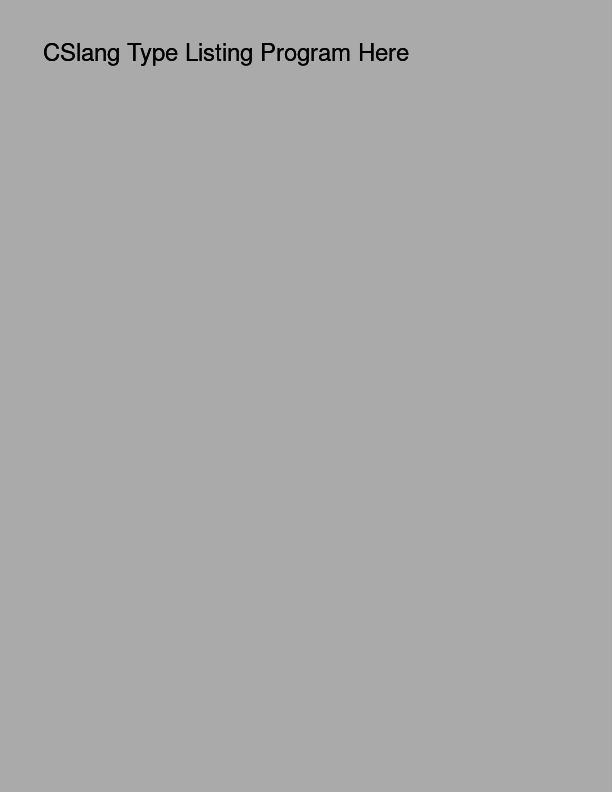
\includegraphics[scale=.30, frame]{images/typelisting}
  \caption{}
  \label{fig:typelisting}
\end{figure}

\begin{figure}
  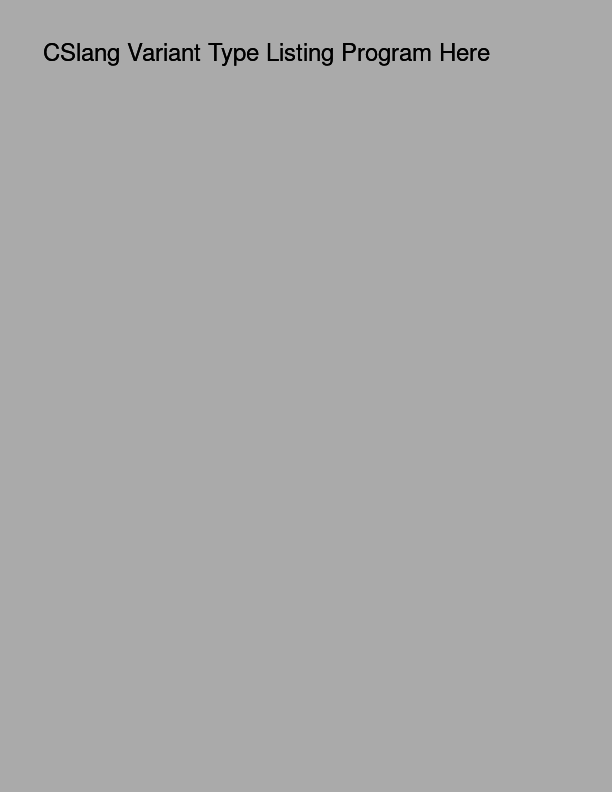
\includegraphics[scale=.30, frame]{images/varianttypes}
  \caption{}
  \label{fig:varianttypes}
\end{figure}

Figure~\ref{fig:bigprogram} shows a complete CSlang program that matches,
and allows for the manipulation of, a sequence of system calls that
facilitates the retrieval of data from a webserver and its storage to a
file on disk.  Such a sequence may be found in programs like {\tt wget} or
{\tt curl}.

Lines 1 through 4 of this program define constructors for the types, {\tt
socket}, {\tt connect}, {\tt send}, {\tt recv}, {\tt read}, and {\tt
write}.  Each of these types corresponds to a system call involved in the
target sequence and the system call parameters we will used to refine the
specific calls to be matched from a system call listing.


Lines 6 through 10 define each define a transducer state that may only be
entered upon encountering a system call with parameters matching the values
defined in the statement....


Figure~\ref{fig:varianttypes} shows an analogous program to the one show in
figure~\ref{fig:bigprogram}.  The purpose of this second program is to
illustrate how CSlang's variant types can be used to more flexibly define a
sequence of system calls.  This is particularly useful when a given task
can be accomplished by more than one system call.  For example, consider
the type {\tt allread} defined on line XXX.  Whenever a statement defines a
state that accepts allread it may be entered upon encountering either a
{\tt read} or {\tt recv} call as these system calls may both be used to
read data from a socket file descriptor (though with slightly different
parameters).  A similar situation can be observed with the type {\tt
allselect}.  Statements accepting allselect may be entered with any of {\tt
poll}, {\tt epoll}, or {\tt select}.  By defining these types in this
manner, a program can be constructed to accept a wider range of sequences
that are all performing the same operation described the first program but
using different system calls.
